\documentclass[11pt]{article}
\usepackage[margin=1in]{geometry}
\usepackage{pdfpages}
\usepackage[colorlinks=true,linkcolor=blue!50!black]{hyperref}

\hypersetup{
  pdftitle={Ginibre Q3 for the adjoint-generated cone: unified submission},
  pdfauthor={Leslie P. Polzer}
}

\begin{document}

\begin{titlepage}
\centering
{\LARGE Ginibre's $Q_3$ condition for the adjoint-generated cone\par}
\vspace{1.2em}
{\Large Unified referee submission\par}
\vspace{2em}
{\large Leslie P. Polzer\par}
\vfill
\begin{minipage}{0.82\textwidth}
This single reader artifact contains the complete formal proof.  Pages after
this guide reproduce, in order:
\begin{enumerate}
\item Parts I--II: the self-contained two-minus adjoint-character theorem,
classification closure, and exact finite-certificate contracts;
\item Part III: the higher-minus hierarchy and promotion to every finite tuple
from the closed multiplicative convex cone generated by the adjoint character.
\end{enumerate}
The optional \texttt{paper\_full.pdf} derivation archive is not part of the
proof and is not required to read or verify any theorem.  Executable evidence,
authenticated transcripts, and implementation notes remain in the companion
artifact repository and are indexed from the two included parts.
\end{minipage}
\vfill
{\large July 2026\par}
\end{titlepage}

% The included PDFs retain their own visible page numbers; suppress wrapper
% page anchors to avoid duplicate destination names at each embedded page 1.
\hypersetup{pageanchor=false}

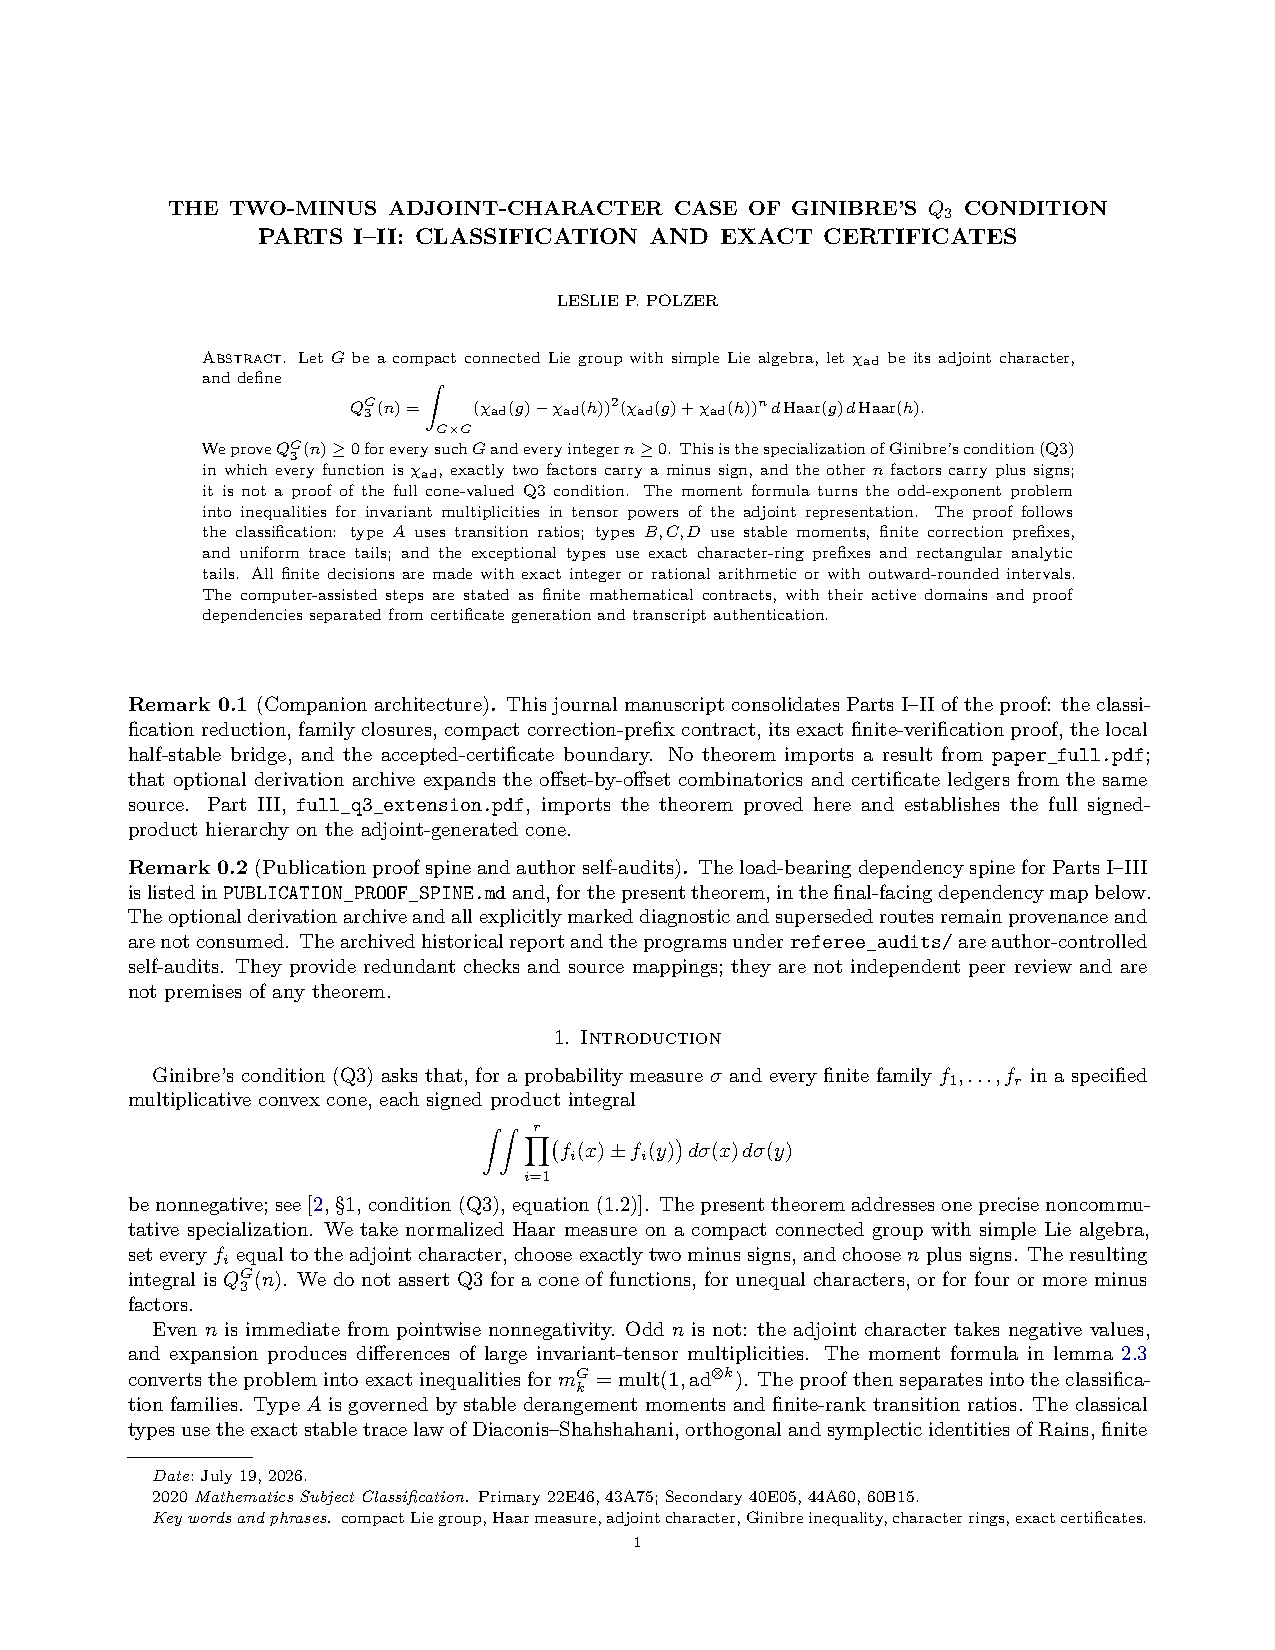
\includepdf[
  pages=-,
  pagecommand={},
  addtotoc={1,part,1,{Parts I--II: the two-minus theorem},parts12}
]{paper.pdf}

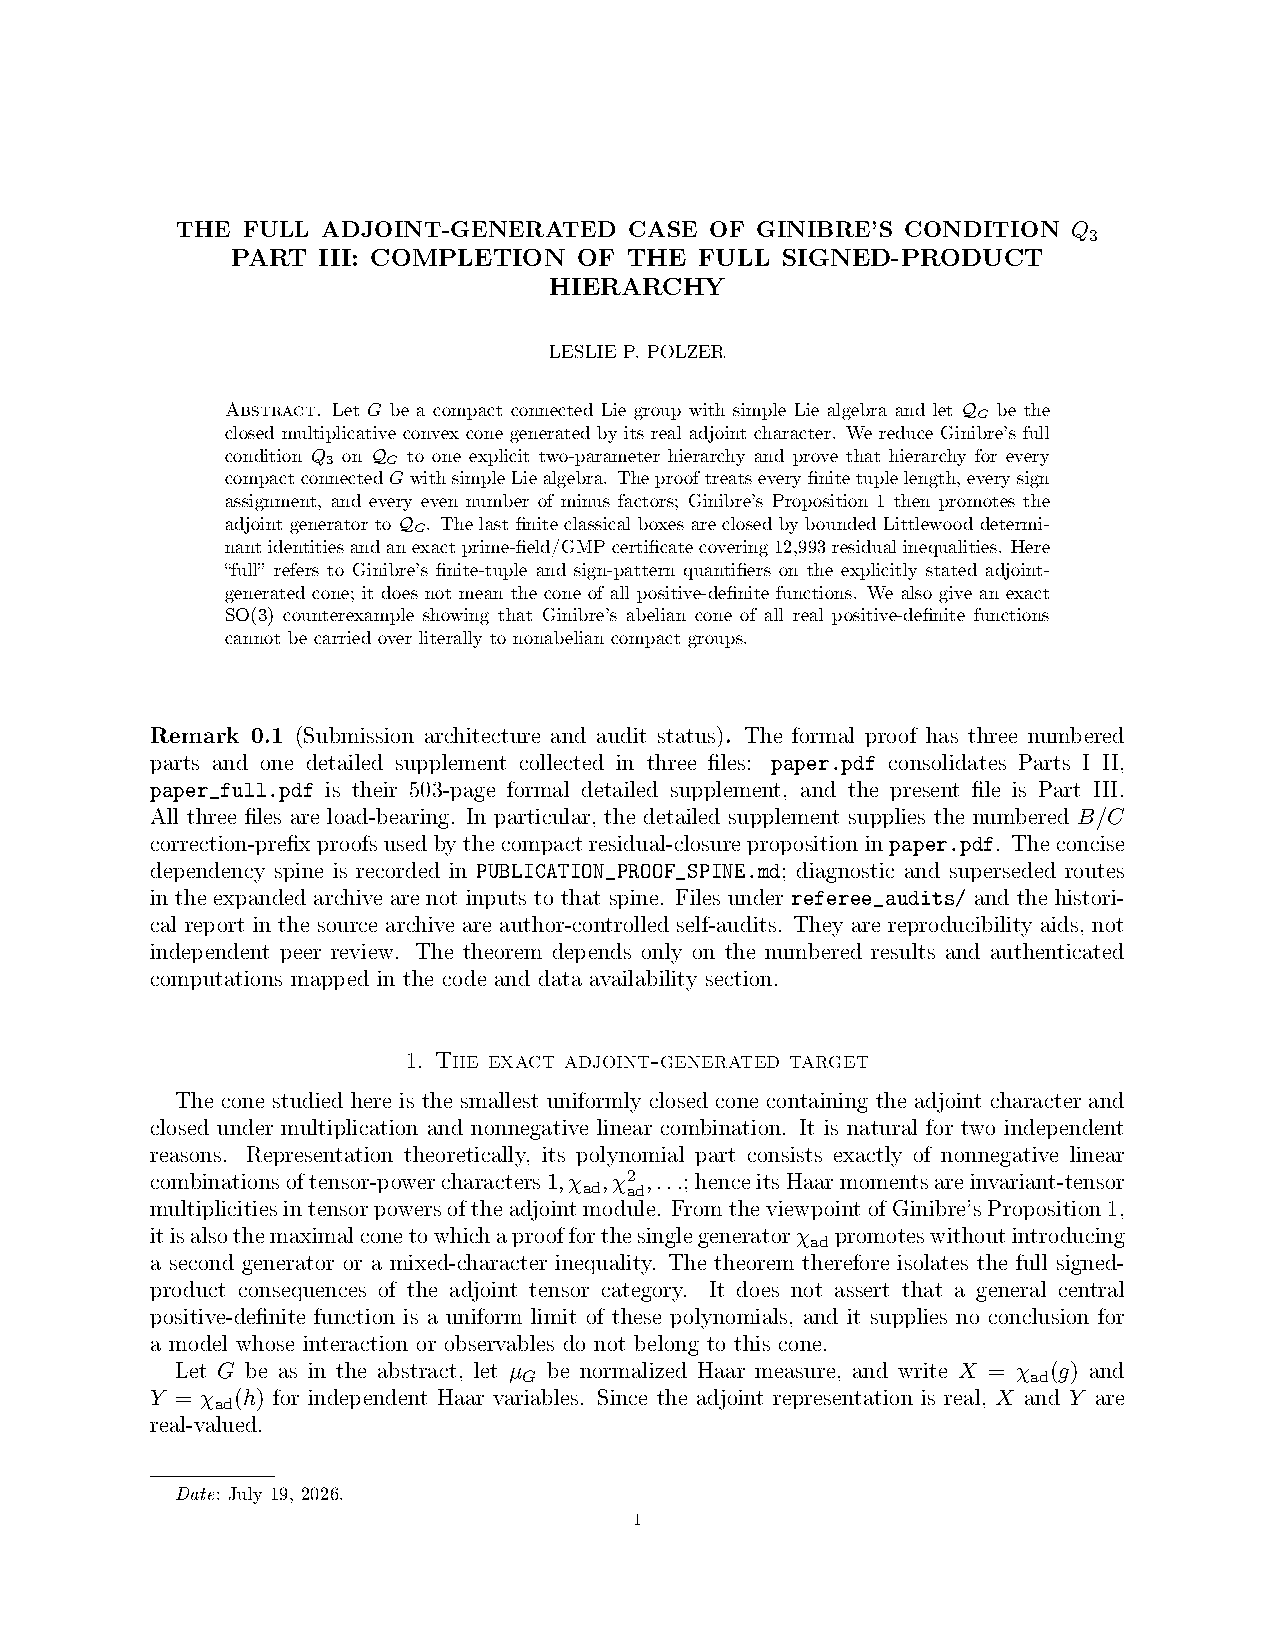
\includepdf[
  pages=-,
  pagecommand={},
  addtotoc={1,part,1,{Part III: the adjoint-generated cone},part3}
]{full_q3_extension.pdf}

\end{document}
